\documentclass[../setup.tex]{subfiles}
\graphicspath{{../images}}

\begin{document}

\title{Probability}
\author{Julian Dominic}
\date{\today}
\pagenumbering{gobble}
\maketitle
\clearpage

\tableofcontents
\pagenumbering{gobble}
\clearpage

\pagenumbering{arabic}
\setcounter{page}{1}

\section{Probability}

\subsection{Probability of an Event}
\begin{theorem}[Probability of an Event]
Let $A$ be an event and $S$ be the sample space.
\[ \textup{P}(A) = \frac{\text{No. of outcomes event occurs}}{\text{No. of possible outcomes}} = \frac{\textup{n}(A)}{\textup{n}(S)} \]
It is important to note that all probabilities are either \textbf{zero} or \textbf{positive} while less than 1. Thus we can say that,
\[ 0 \leq \textup{P}(A) \leq 1 \]
\end{theorem}

\begin{remark} 
It is also important to note that the sum of all possible events is equal to 1. \[ \sum_{\text{all } n} \textup{P}(X=n) = 1 \]
\end{remark}

\subsection{Complimentary Events}
\begin{theorem}[Complimentary Events]
We denote the compliment of an event by an \textit{apostrophe}, \texttt{'} ; We say that the compliment of event $A$ is $A'$. Compliments are other events that occur that are \textbf{not} $A$. Let $A$ be the event that I ate an apple, $A'$ will be the event that I did \textbf{not} eat an apple. If $A$ is the only event, then the total sample space will be made up of only $A$ and $A'$. Thus, we can say that,
\[ \label{compliment} \textup{P}(A) + \textup{P}(A') = 1\]
\end{theorem}

In Mathematics, we use special symbols to represent the words ``or'' and ``and'' which are ``$\cup$'' and ``$\cap$'' respectively. When we read certain expressions such as $\textup{P}(A \cup B)$, we read it as 'Probability of the \textit{union} of $A$ and $B$' while $\textup{P}(A \cap B)$ is read as 'Probability of the \textit{intersection} of $A$ and $B$'. Though some may identify ``$\cup$'' as add and ``$\cap$'' as multiply.
\begin{remark}
It is also important to note that the word ``or'' has the additive note of ``inclusive''. This means that $\textup{P}(A \cup B)$ says that we want the probability that either $A$, $B$ or \textit{both} occurs.
\end{remark}

\subsection{Principle of Inclusion and Exclusion}
\begin{theorem}[Principle of Inclusion and Exclusion]
Let $A$ and $B$ be events in the sample space.
\begin{align*} 
\textup{P}(A \text{ or } B) &= \textup{P}(A \cup B) \\
&= \textup{P}(A) + \textup{P}(B) - \textup{P}(A \cap B)
\end{align*}
Similarly,
\begin{align*} 
\textup{P}(A \text{ and } B) &= \textup{P}(A \cap B) \\
&= \textup{P}(A) + \textup{P}(B) - \textup{P}(A \cup B)
\end{align*}
\end{theorem}

\subsection{Conditional Probability}
\begin{theorem}[Conditional Probability]
Conditional probabilities are when we are asked to find a certain probability of an event \textit{given} that another event has already occured.
\[ \textup{P}(A | B) = \frac{\textup{P}(A \cap B)}{\textup{P}(B)} \]
We read ``$|$'' as ``given''; $\textup{P}(A | B)$ is read as ``Probability of event $A$ given $B$''.
\end{theorem}

\subsection{Mutually Exclusive Events}
\begin{theorem}[Mutually Exclusive Events]
Mutually Exclusive Events are events that \textbf{cannot happen at the same time} (simultaneously). For example, in a standard deck of 52 poker cards, it is impossible to draw a card that is both red and clubs --- because clubs are all black. Thus, this means that the \textit{intersection} of such events is \textbf{zero}.
\[ \textup{P}(A \cap B) = 0 \]
Knowing this, we can see that
\[ \textup{P}(A \cup B) = \textup{P}(A) + \textup{P}(B) \]
also,
\[ \textup{P}(A | B) = 0 \text{ (Since B occurs, A wont occur, vice versa)}\] 
\end{theorem}

\subsection{Independent Events}
\begin{theorem}[Independent Events]
Independent events are events where the occurence of one \textbf{does not affect} the others.
\[ \textup{P}(A \cap B) = \textup{P}(A) \times \textup{P}(B) \]
Knowing this, we can see that
\[ \textup{P}(A | B) = \textup{P}(A) \]
\end{theorem}
\begin{proof}
\begin{align*} 
\textup{P}(A | B) &= \frac{\textup{P}(A \cap B)}{\textup{P}(B)} \\
&= \frac{\textup{P}(A) \times \textup{P}(B)}{\textup{P}(B)} \\
&= \frac{\textup{P}(A) \times \cancel{\textup{P}(B)}}{\cancel{\textup{P}(B)}} \\
&= \textup{P}(A)
\end{align*}
\end{proof}
\clearpage

\subsection{Other Useful Formulas}
\begin{proposition}[Other useful formulas]
\[ \textup{P}(A \cup B) = 1 - \textup{P}(A' \cap B') \]
\[ \textup{P}(A \cap B) = 1 - \textup{P}(A' \cup B') \]
\[ \textup{P}(A) = \textup{P}(A \cap B) + \textup{P}(A \cap B') \]
\[ \textup{P}(A | B) + \textup{P}(A' | B) = 1 \]
\end{proposition}
\begin{proof} 
\textit{Left as an exercise for the reader.} \\
Do draw the venn diagrams! They are a huge help.
\end{proof}

\begin{figure}[H]
    \centering
    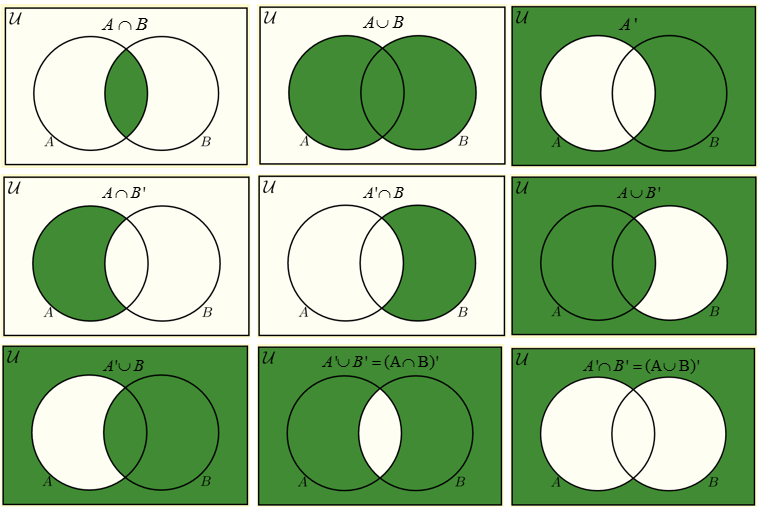
\includegraphics[scale=0.6]{Venn Diagram.jpg}
    \caption{Source from Google}
\end{figure}

\section{Probability Distributions}
In this section, we will cover two overarching types of Random Variables (R.V.) and the different types of probabilistic distributions they have.
\subsection{Random Variables}
\begin{enumerate}
	\item \textbf{Discrete Random Variable (DRV)} \begin{itemize} \item DRVs mainly consists of numbers that are \emph{exact}. It may consist of numbers such as \{0, 1, 2, 3, 4, 5, ...\} or even \{0, 0.5, 1.5, 2.5, 3.5, ...\}. \item Binomial and Poisson Distributions will be covered. \end{itemize}
	\item \textbf{Continuous Random Variable (CRV)} \begin{itemize} \item CRVs mainly consists of numbers that are never ending (irrational) but not all of them have to be such. It can consists of the numbers stated earlier in the DRV example but it will never be able to yield the exact value --- meaning that for a CRV $X$, $\textup{P}(X=1)$ is 0. A CRV is only valid for a \emph{range of values} such as $\textup{P}(1 \leq X \leq 2)$.  \item Only the Normal Distribution will be covered. \end{itemize}
\end{enumerate}
\begin{remark} Without going into too much details about the math, take note of the following which is \textbf{only true for a CRV},
\[ \textup{P}(a \leq X \leq b) = \textup{P}(a < X \leq b) = \textup{P}(a \leq X < b) = \textup{P}(a < X < b) \] \end{remark}
\begin{remark} It is also important to note that the `input' (your $X$ value) of both the DRVs and CRVs  can be \textit{negative}. However, the `output' (your probability) \textbf{must} be \textit{positive}. Also, all DRVs must start from 0 unless stated otherwise. \end{remark}

\subsection{Some Terminology}
While the following terminology is more widely used in other fields of statistics other than probability, it is still important to know what they mean for learning the distributions.

\begin{tabular}{| l | l | c |}
\hline 
Term & Meaning & Symbol \\
\hline 
& & \\
Mode & Highest probability/Appeared the most & NA.  \\
& & \\
Expectation & Mean/Average & $\mu$ or $\bar{x}$ or E$(X)$ \\
& & \\
Standard Deviation & How much each data point defers from each other & $\sigma$ \\
& & \\
Variance & How far each data is spread out from the mean value & $\sigma^2$ or Var$(X)$ \\
\hline 
\end{tabular} 
\clearpage

\subsection{How do we calculate Expectation and Variance?}

\begin{lemma}[Expectation]
To find the Expectation of a DRV $X$, we will have to do,
\[ \textup{E}(X) = \sum_{\text{all } x} x\textup{P}(X = x) \]
this that means for each $x$ value, we have to multiply it with its corresponding probability then add it all up. \\ \\
In general, if we want to find the expectation for another variable but it is still in terms of $X$, $Y=2X$,
\[ \textup{E}(g(X)) = \sum_{\text{all } x} g(x)\textup{P}(X = x) \]
where $g(x) = Y = 2X$. \\ \\
For a CRV, it gets more complicated because it requires \textbf{calculus}. \textit{(Skip if not needed)}
\[ \textup{E}(X) = \int_{\mathbb{R}} xf(x) \textup{d}x \]
\[ \textup{E}(g(X)) = \int_{\mathbb{R}} g(x)f(x) \textup{d}x \]
\end{lemma}

\begin{lemma}[Variance]
\[ \textup{Var}(X) = \textup{E}(X - \mu)^2 = \textup{E}(X^2) - [\textup{E}(X)]^2 \]
\end{lemma}
\begin{proof}
\begin{align*}
\textup{Var}(X) &= \textup{E}(X - \mu)^2 \\
&= \textup{E}(X^2 - 2\mu X + \mu^2) \\
&= \textup{E}(X^2) + \textup{E}(- 2\mu X) + \textup{E}(\mu^2) \\
&= \textup{E}(X^2) - 2\mu \textup{E}(X) + \mu^2 \\
&= \textup{E}(X^2) - 2\mu^2 + \mu^2 \\
&= \textup{E}(X^2) - [\textup{E}(X)]^2 \\
\end{align*}
\end{proof}
\clearpage

\subsubsection{Properties of Expectation and Variance}
\begin{tabular}{| c | c |}
\hline
& \\
E$(a)=a$ & Var$(a)=0$  \\
& \\
E$(aX)=a$E$(X)$ & Var$(aX)=a^2$Var$(X)$ \\
& \\
E$(aX\pm b)=a$E$(X) \pm b$ & Var$(aX \pm b)=a^2$Var$(X)$ \\
& \\
E$(X_1 + \dots + X_n)=$E$(X_1)+\dots + $E$(X_n)=n$E$(X)$ & Var$(X_1 + \dots + X_n)=$Var$(X_1)+\dots + $Var$(X_n)=n$Var$(X)$ \\
& \\
E$(aX\pm bY)=a$E$(X) \pm b$E$(Y)$ & Var$(aX \pm bY)=a^2$Var$(X) + b^2$Var$(Y)$ \\
& \\
\hline
\end{tabular}

\section{Binomial Distribution}
\begin{theorem}[Binomial Distribution]
To say that $X$ follows a Binomial Distribution, we write,
\[ X \sim \textup{B}(n, p) \] 
where $n$ is the number of trials and $p$ is the probability of success. \\
The probability distribution function (pdf) of a Binomial Distribution is,
\[ \text{\textbf{pdf}} = \textup{P}(X = x) = \binom{n}{x} p^x (1-p)^{n-x} \]
\end{theorem}

\subsection{Expectation, Variance, Standard Deviation}
\begin{enumerate}
	\item Expectation \[ \textup{E}(X) = \mu = \bar{x} = np \]
	\item Variance \[ \textup{Var}(X) = \sigma^2 = np(1-p) \]
	\item Standard Deviation \[ \sigma = \sqrt{np(1-p)} \]
\end{enumerate}

\subsection{Conditions for a Binomial Distribution}
\begin{enumerate}
	\item There a $n$ \textbf{independent} trials,
	\item Each trial has \textbf{exactly two possible outcomes}: ``success'' or ``failure'',
	\item The probability of a success, $p$, is always constant (the same) for all trials. 
\end{enumerate}
\begin{remark} If you think about it, without $n$ fixed trials, how are we going to calculate any of the statistics --- expectation, variance, and std. dev? 
\end{remark}

\section{Poisson Distribution}

\begin{theorem}[Poisson Distribution]
To say that $X$ follows a Poisson Distribution, we write,
\[ X \sim \textup{Po}(\lambda) \]
where $\lambda$ is the mean number of occurences. \\
The pdf of a Poission Distribution is,
\[ \text{\textbf{pdf}} = \textup{P}(X = x) = e^{-\lambda}\frac{\lambda^x}{x!} \]
\end{theorem}

\subsection{Expectation, Variance, Standard Deviation}
\begin{enumerate}
	\item Expectation \[ \textup{E}(X) = \mu = \bar{x} = \lambda \]
	\item Variance \[ \textup{Var}(X) = \sigma^2 = \lambda \]
	\item Standard Deviation \[ \sigma = \sqrt{\lambda} \]
\end{enumerate}

\begin{remark} One special way to check if it's really a poisson distribution is to see whether \[ \textup{E}(X) \approx \textup{Var}(X) \]
\end{remark}

\subsection{Conditions for a Poisson Distribution}
\begin{enumerate}
	\item The events occur randomly and are independent of each other in a given interval of time or space,
	\item The events occur singly (one at a time) --- no two events can occur at the same instant; only one,
	\item The mean number of occurences of events, $\lambda$, is constant throughout the interval. 
\end{enumerate}

\subsection{Additive Property}
\begin{theorem}[Additive Property]
If $X \sim$ Po$(\lambda_x)$ and $Y \sim$ Po$(\lambda_y)$, and $X$ and $Y$ are \textbf{independent}, then $X + Y \sim$ Po$(\lambda_x + \lambda_y)$.
\end{theorem}
\clearpage

\section{Normal Distribution}
Even though the Normal Distribution has its \textbf{pdf}, I will not be covering it in here because you will most likely be converting it to the Standard Normal Distribution and using a z-score table.
\begin{theorem}[Normal Distribution]
To say that $X$ follows a Normal Distribution, we write,
\[ X \sim  \textup{N}(\mu, \sigma^2) \]
where $\mu$ and $\sigma^2$ are the mean and variance respectively.
\end{theorem}

\subsection{Additive Property}
\begin{theorem}[Additive Property]
If $X\sim $\textup{ N}$(\mu_x, \sigma_x^2)$ and $Y\sim $\textup{ N}$(\mu_y, \sigma_y^2)$ are \textbf{independent}, then $aX \pm bY\sim $\textup{ N}$(\mu_x \pm \mu_y, \sigma_x^2 + \sigma_y^2)$. 
\end{theorem}

\subsection{Standardised Distribution}
\begin{theorem}[Standard Normal Distribution (Standardised Distribution)]
The Standard Normal Distribution (Standardised Distribution) is unique because its mean is $0$ and variance is $1$. \\
We say that $Z$ is the Standardised Distribution,
\[ Z \sim \textup{N}(0, 1) \] \\
The special thing about the Standardised Distribution is that any other Normal Distriubtion can be transformed into it through `standardisation',
\[ Z = \frac{X-\mu}{\sigma} \]
where $\mu$ and $\sigma$ are the mean and variance of the Normal Distribution $X$.
\end{theorem}

\subsection{Area under the Normal Curve}
Due to the unique shape of the Normal Distribution Curve (Normal Curve), it is symmetrical about the mean, $\mu$. We have the following properties, 
\begin{enumerate}
	\item P$(X < \mu) =$ P$(X > \mu) = 0.5$
	\item P$(X > a) = 1 -$ P$(X < a)$
	\item P$(X < \mu + a) =$ P$(X > \mu - a)$
\end{enumerate} 
\begin{proof} \textit{This is left as an exercise for the reader.} \\ Draw out the curve, mark out the points and see the magic!
\end{proof}

\subsection{Sample Mean Distribution}
\begin{theorem}[Sample Mean Distribution]
We denote $\bar{X}$ to be the Sample Mean of $X$,
\[ \bar{X} = \frac{X_1 + \dots + X_n}{n} \]
To say that $\bar{X}$ follows a Normal Distribution, we write,
\[ \bar{X} \sim \textup{N}\left(\mu, \frac{\sigma^2}{n}\right) \]
where E$\left(\bar{X}\right)=\mu$ and Var$\left(\bar{X}\right)=\frac{\sigma^2}{n}$. 
\end{theorem}
\begin{proof} . \\
For the expectation,
\begin{align*}
\textup{E}\left(\bar{X}\right) &= \textup{E}\left(\frac{X_1 + \dots + X_n}{n}\right) \\
&= \frac{1}{n}\textup{E}(X_1 + \dots X_n) \\
&= \frac{1}{n} \times n\mu \\
&= \mu
\end{align*}

For the variance,
\begin{align*}
\textup{Var}\left(\bar{X}\right) &= \textup{Var}\left(\frac{X_1 + \dots + X_n}{n}\right) \\
&= \frac{1}{n^2}\textup{Var}(X_1 + \dots X_n) \\
&= \frac{1}{n^2} \times n\sigma^2 \\
&= \frac{\sigma^2}{n}
\end{align*}
\end{proof}

\subsection{Central Limit Theorem}
\begin{theorem}[Central Limit Theorem (CLT)]
As long as the sample size, $n$, is greater than $30$ (might be 50; depending on school), then the disstirbution can be approximated to a Normal Distribution. \\
If $X_1, X_2, \dots, X_n$ are \textbf{unknown} distributions, each with mean $\mu$ and variance $\sigma^2$,
\[ X_1 + X_2 + \dots + X_n \sim \textup{N}(n\mu, n\sigma^2) \]
\[ \bar{X} \sim \textup{N}\left(\mu, \frac{\sigma^2}{n}\right) \]
\end{theorem}
\clearpage

\section{Examples}
\subsection{Example 1}
\begin{example}[9740/2013/02/Q8]
For events $A$ and $B$, it is given that P$(A)=0.7$, P$(B|A')=0.8$, and P$(A|B')=0.88$ . Find
\begin{itemize}
	\item P$(B \cap A')$
	\item P$(A' \cap B')$
	\item P$(A \cap B)$
\end{itemize}
\end{example}
\begin{proof}. \\
For the first part, we know that \[ \textup{P}(B|A') = \frac{\textup{P}(B\cap A')}{\textup{P}(A')} \]
By rearranging, we get,
\begin{align*}
\textup{P}(B \cap A') &= \textup{P}(B|A') \times \textup{P}(A') \\
&= \textup{P}(B|A') \times (1 - \textup{P}(A)) \\
&= 0.8 \times (1 - 0.7) \\
&= 0.24 \\
\end{align*}
For the second part, we know that \[ \textup{P}(B|A') = 1 - \textup{P}(B'|A') \] 
By rearranging, we get,
\begin{align*}
\textup{P}(B'|A') &= 1 - \textup{P}(B|A') \\
&= 0.2 \\
\implies \frac{\textup{P}(B' \cap A')}{\textup{P}(A')} &= 0.2 \\
\implies \textup{P}(A' \cap B') &= 0.2 \times (1-\textup{P}(A)) \\
&=  0.2 \times (1-0.7) \\
& = 0.06
\end{align*}
For the last part, 
\begin{align*}
\textup{P}(A \cap B) &= \textup{P}(A \cup B) - \left(\textup{P}(B \cap A') + \textup{P}(A \cap B')\right) \\
&= \left(1 - \textup{P}(A' \cap B')\right) - \left(0.24 + \textup{P}(A|B') \times \textup{P}(B')\right) \\
&= (1 - 0.06) - \left(0.24 + 0.88\times \frac{\textup{P}(A' \cap B')}{\textup{P}(A'|B')} \right) \\
&= 0.94 - \left(0.24 + 0.88 \times \frac{0.06}{1-0.88} \right) \\
&= 0.26
\end{align*}
\end{proof}
\clearpage

\subsection{Example 2}
\begin{example}
A hand of $4$ cards is randomly dealt \textbf{without replacement} from a standard deck of 52 playing cards. Find the probability that 
\begin{itemize}
	\item there is at least an ace,
	\item there are exactly 3 ``Spades'' cards,
	\item all the cards are even numbered cards.
\end{itemize}
\end{example}
\begin{proof} . \\
For the first part,
\begin{align*}
\textup{P}(\text{there is at least an ace}) &= \textup{P}(1 \textup{ ace}) + \textup{P}(2 \textup{ aces}) + \textup{P}(3 \textup{ aces}) + \textup{P}(4 \textup{ aces}) \\
&= 1 - \textup{P}(\textup{no aces}) \\
&= 1 - \left(\frac{48}{52}\cdot\frac{47}{51}\cdot\frac{46}{50}\cdot\frac{45}{49}\right) \\
&= 0.281 \ (3. \textup{ sf})
\end{align*}
For the second part,
\begin{align*}
\textup{P}(\text{there are exactly 3 ``Spades'' Cards}) &= \frac{13}{52} \cdot \frac{12}{51} \cdot \frac{11}{50} \cdot \frac{39}{49} \cdot 4 \\
&= 0.0412 \ (3. \textup{ sf})
\end{align*}
For the last part,
\begin{align*}
\textup{P}(\text{all the cards are even numbered cards}) &= \frac{5 \times 4}{52} \cdot \frac{5 \times 4 - 1}{51} \cdot \frac{5 \times 4 - 2}{50} \cdot \frac{5 \times 4 - 3}{49} \\
&= 0.0179 \ (3. \textup{ sf})
\end{align*}
\end{proof}
\begin{remark} Notice that for the first part, instead of manually calculating the probabilities for the multiple aces, I just did $1-$P$($no aces$)$. This is only possible because of \ref{compliment} --- Complimentary Events. Let $A$ be the event that there is at least one ace. $A'$ will be the event that there is no ace.
\end{remark}
\clearpage

\subsection{Example 3}
\begin{example}[2017/SAJC/Prelim/II/6]
A fairground game involves trying to hit a moving target with a gunshot. A round consists of \textbf{maximum} of 3 shots. Ten points are scored if a player hits the target. The \textbf{round ends immediately} if the player misses a shot. Linda has a 60\% to hit the target in a single shot. All shots taken are independent of one another.
\begin{itemize}
	\item Find the probability that Linda scores $30$ points in a round \\ \\
\textbf{The random variable $X$ is the number of points Linda scores in a round.}
	\item Find the probability distribution of $X$,
	\item Find the mean and variance of $X$,
	\item A game consists of $2$ rounds. Find the probability that Linda scores more points in round $2$ than in round $1$.
\end{itemize}
\end{example}
\begin{proof} . \\
For the first part,
\begin{align*}
\textup{P}(\text{Linda scores 30 points in a round}) &= \textup{P}(3 \text{ hits}) \\
&= (0.6)^3 \\
&= 0.216 \\
\end{align*}
For the second part, \\
\begin{tabular}{| c | c | c | c | c |}
\hline
$x$ & $0$ & $10$ & $20$ & $30$ \\
\hline
\textup{P}$(X=x)$ & 0.4 & 0.24 & 0.144 & 0.216 \\
\hline
\end{tabular}
For the third part,
\begin{align*}
\textup{E}(X) &= \sum_{\text{all }x} x\textup{P}(X=x) \\
&= 0\cdot\textup{P}(X=0) + 10\cdot\textup{P}(X=1) + 20\cdot\textup{P}(X=2) + 30\cdot\textup{P}(X=3) \\
&= 10\cdot 0.24+ 20\cdot 0.144 + 30\cdot 0.216 \\
&= 11.76 \\ \\
\textup{Var}(X) &= \textup{E}(X^2) - [\textup{E}(X)]^2 \\
&= \sum_{\text{all }x} x^2\textup{P}(X=x) - (11.76)^2 \\
&= 0^2\cdot\textup{P}(X=0) + 10^2\cdot\textup{P}(X=1) + 20^2\cdot\textup{P}(X=2) + 30^2\cdot\textup{P}(X=3) - (11.76)^2 \\
&= 10^2\cdot 0.24 + 20^2\cdot 0.144 + 30^2\cdot 0.216 - (11.76)^2 \\
&= 137.7024 \\
\end{align*}
\clearpage
For the last part, let $X_1$ be the number of points scored by Linda in Round $1$ and let $X_2$ be the number of points scored by Linda in Round $2$.
\begin{align*}
\text{Required Probability} &= \textup{P}(X_1=0\cap X_2\geq10)+\textup{P}(X_1=10\cap X_2\geq20)+ \textup{P}(X_1=20\cap X_2=30) \\
&=\textup{P}(X_1=0)\textup{P}(X_2\geq10) + \textup{P}(X_1=10)\textup{P}(X_2\geq20)+ \textup{P}(X_1=20)\textup{P}(X_2=30) \\
&= 0.4\cdot(1-0.4) + 0.24\cdot(0.144+0.216) + 0.144\cdot0.216 \\
&= 0.357504
\end{align*}
\end{proof}

\subsection{Example 4}
\begin{example}[2012/CJC/Prelim/II/8]
On average, the probability that John receives at least one Short Message (SMS) on his mobile phone in any given $30$-minutes period is $0.95$. A school day consists of $14$ such periods of $30$ minutes each. The number of periods in which John receives at least one SMS in a school day is the random variable $X$.
\begin{itemize}
	\item State, in the context of this question, the assumptions needed to model $X$ by a binomial distribution.
	\item Explain why one of the assumptions stated in the first part may not hold in this context. \\ \\
\textbf{Assume now that these assumptions in the first part hold.}
	\item Find the probability that in a school day, John receives at least one SMS in at least $3$ periods but not more than $12$ periods.
\end{itemize} 
\end{example}
\begin{proof} . \\
For the first part, the assumptions are:
\begin{enumerate}
	\item The number of SMSes that John receives (none or otherwise) in each $30$ minute period is independent of the number of SMSes John received in other $30$ minute periods.
	\item The probability that John receives at least one SMS in a $30$ minute period is the same for any such $30$ minute periods.
\end{enumerate}
For the second part, assumption $(2)$ may not hold as the people who contact John will do so at their own convenience. It is unlikely that there is an equal chance of him receiving at least one SMS for each $30$ minute period. \\ \\
For the last part, $X \sim \textup{B}(14, 0.95)$
\begin{align*}
\textup{P}(3\leq X\leq12) &= \textup{P}(X\leq12) - \textup{P}(X\leq2) \\
&= [1 - (\textup{P}(X=13) + \textup{P}(X=14))] - (\textup{P}(X=0) + \textup{P}(X=1) + \textup{P}(X=2)) \\
&= 1 -\left(\binom{14}{13}(0.95)^{13}(1-0.95)^1 + (0.95)^{14}\right) \\ &- \left((1-0.95)^{14} + \binom{14}{1}(0.95)(1-0.95)^{13} + \binom{14}{2}(0.95)^2(1-0.95)^{12}\right) \\
&= 0.153 \ (3. \text{ sf})
\end{align*}
\end{proof}
\clearpage

\subsection{Example 5}
\begin{example}[intmath.com]
A life insurance salesman sells on the average $3$ life insurance policies per week. Assume that the amount of policies sold can be modelled by a poisson distribution.
\begin{itemize}
	\item Some policies
	\item $2$ or more policies but less than $5$ policies
	\item Assuming that there are $5$ working days per week, what is the probability that in a given day he will sell one policy?
\end{itemize}
\end{example}
\begin{proof} . \\
For the first part, ``Some policies'' means ``at least $1$ policy''. 
\begin{align*}
\textup{P}(X\geq1) &= 1 - \textup{P}(X=0) \\
&= e^{-3}\left(\frac{3^0}{0!}\right) \\
&= 0.0498 (3. \text{ sf})
\end{align*}
For the second part,
\begin{align*}
\textup{P}(2\leq X < 5) &= \textup{P}(2\leq X\leq4) \\
&= \textup{P}(X=2) + \textup{P}(X=3) + \textup{P}(X=4) \\
&= e^{-3}\left(\frac{3^2}{2!}\right) + e^{-3}\left(\frac{3^3}{3!}\right) + e^{-3}\left(\frac{3^4}{4!}\right) \\
&= 0.616 (3. \text{ sf})
\end{align*}
For the third part, average number of policies sold per day is $$\frac{3}{5} = 0.6$$
\begin{align*}
\textup{P}(Y=1) &= e^{-0.6}\left(\frac{0.6^1}{1!}\right) \\
&= 0.329 (3. \text{ sf})
\end{align*}
\end{proof}
\clearpage

\subsection{Example 6}
\begin{example}[examsolutions.net]
The heights of adult females are normally distributed with mean $160$cm and standard deviation $8$cm.
\begin{itemize}
	\item Find the probability that a randomly selected adult female has a height greater than $170$cm. \\ \\
\textbf{Any adult female whose height is greater than $170$cm is defined as tall.}
	\item An adult female is chosen at random. Given that she is tall, find the probability that she has a height greater than $180$cm.
	\item Given that half of tall adult females have a height greater than $h$ cm Find the value of $h$.
\end{itemize}
\end{example}
\begin{proof} 
\textbf{All answers will come from a z-score table.} \\
For the first part, we are know that $X \sim \textup{N}(160, 8^2)$.
\begin{align*}
\textup{P}(X > 170) &= \textup{P}\left(Z > \frac{170-160}{8} \right) \\
&= \textup{P}(Z > 1.25) \\
&= 0.5 - 0.3944 \\
&= 0.1056
\end{align*}
For the second part,
\begin{align*}
\textup{P}(X>180 | X>170) &= \frac{\textup{P}(X>180)}{P(X>170)} \\
&= \frac{\textup{P}\left(Z > \frac{180-160}{8}\right)}{\textup{P}(X>170)} \\
&= \frac{\textup{P}(Z>2.5)}{\textup{P}(X>170)} \\
&= \frac{0.5-0.4938}{0.1056} \\
&= 0.0587 \ (3. \text{ sf})
\end{align*}
For the third part,
\begin{align*}
\textup{P}(X>h) &= \frac{0.10565}{2} \\
\implies \textup{P}(X<h) &= 1 - \frac{0.10565}{2} \\
\implies \textup{P}\left(Z<\frac{h-160}{8}\right) &= 1 - \frac{0.10565}{2} \\
&= 0.947175 \\
\implies \textup{P}\left(0<Z<\frac{h-160}{8}\right) &= 0.447175
\end{align*}
\text{From the z-score table, for the value of $0.447175$, \textbf{z $\approx$ 1.62}} \\
$$\implies \frac{h-160}{8} = 1.62 \implies h = 172.96$$
\end{proof}


\end{document}